%%
%% 
%% 
\documentclass[10pt]{article}
\usepackage{graphicx}
\DeclareGraphicsExtensions{.pdf,.png,.eps,.jpg}
%\graphicspath{{./figures/}{../support/}}
%\usepackage{times}
\usepackage{listings}
\usepackage[hyphens]{url}
\usepackage{hyperref}
\usepackage{xcolor}
\usepackage{color}
\usepackage{epsfig} 
\usepackage{amssymb}
\usepackage{amsmath}
\usepackage{amsfonts}
\usepackage{floatflt}
\usepackage{wrapfig}
\usepackage{enumitem}
\usepackage{tablefootnote}
\usepackage{eurosym}
\usepackage{pdfpages}
\usepackage{graphicx}
\setcounter{secnumdepth}{5}
\setcounter{tocdepth}{5}


\setlength{\oddsidemargin}{0in}   % 10pt is 1.875 for margins in latex
\setlength{\evensidemargin}{0in}
\setlength{\textwidth}{6.5in}
\setlength{\textheight}{9in}
\setlength{\topmargin}{-0.5in}

\setitemize{leftmargin=*}

\newcommand{\ignore}[1]{}
%\input{remark}
%\remarktrue

\newcommand{\EUCALYPTUS} {\textsc{eucalyptus}}
\newcommand{\eUCALYPTUS} {\textsc{Eucalyptus}}
\newcommand{\NAMENS} {\textsc{FarmingEdge}}
\newcommand{\NAME} {\textsc{FarmingEdge }}

%\thispagestyle{empty}

\title{CSPOT Dataflow Prototype}
\author{Rich Wolski}
\date{\today}

\begin{document}
\maketitle

\section{Introduction}

The basic idea is to create a set of primitives that can be used to implement
a simple data flow language (textually) that can be executed as a script in
some scripting language.  The code that is in \verb+cspot/apps/dataflow+ in
the \verb+release-2.0+ branch is a
small, proof-of-concept prototype.  It is not a general dataflow
implementation but rather an experiment that shows that CSPOT can implement
dataflow computations expressed as directed, acyclic graphs (DAGS).

The following outline assumes that the reader is familiar with CSPOT as it is
described in the CSPOT Technical Report available from
\url{https://www.cs.ucsb.edu/research/tech-reports/2018-01}.

The prototype has the following restrictive properties (compared to a complete
implementation).
\begin{itemize}
\item All DAG nodes (representing computations) have $2$ input edges and $1$
output edge.
\item The only data type that can be conveyed along a DAG edge is a C
double-precision floating point number.  Thus, the prototype only implements
double-precision floating point computations.
\item When a node computation is not commutative with respect to its inputs,
the left input to the operator corresponding to a node must be flagged as
such.
\item The output of a program that has been executed is stored at the end of
the program WooF (see below).  All print statements from within a handler
appear in the output of woofc-namespace. 
\item The $3$ CSPOT dataflow primitives are designed to be called from bash as
a bash script.
\item The prototype only executes a single DAG (there is no iteration or
conditional execution).
\end{itemize}
The directory for the CSPOT dataflow code includes a single bash script --
\verb+quadratic.sh+ -- that computes one of the roots of the quadratic
formula as an example.

\section{The CSPOT Dataflow Components}

The prototype consists of $4$ CSPOT software components: $3$ CSPOT programs 
and $1$ CSPOT handler.
\begin{itemize}
\item \verb+dfinit.c+ is a program that initializes $2$ WooFs that are needed
to execute a program.
\item \verb+dfaddnode.c+ is a program that appends a dataflow node to a WooF
that contains the state of the dataflow program nodes at any time during its
execution.
\item \verb+dfaddoperand.c+ is a program that appends edges to a WooF that
records which edges are ready to transmit their carried operand to a
destination node.
\item \verb+dfhandler.c+ is a CSPOT handler invoked when an edge is added to
the operand WooF.  It executes an algorithm that moves the dataflow program
through its next state transition.
\end{itemize}
The \verb+dfinit+ program initializes or reinitializes the WooFs that are
necessary to execute a DAG and, thus, must be called before any nodes or edges
are added to these WooFs.  

\section{Writing a CSPOT Dataflow Program}

A CSPOT dataflow program, executed as a script, consists of $3$ sections that
must be executed in order.  The script must
\begin{itemize}
\item Call \verb+dfinit+ in the CSPOT namespace where the WooFs are to be
created (i.e. where the program will execute).
\item Call \verb+dfaddnode+ once for each node in the DAG (syntax discussed
below).  Note that the order in which nodes are added does not affect program
correctness but might affect program performance.
\item Call \verb+dfaddoperand+ once for each edge in the DAG that carries an
input to the program itself. The order in which edges are added does not
affect program correctness and likely does not affect program performance.
\end{itemize}
Using \verb+quadratic.sh+ as an example, the code is 

\begin{lstlisting}[language=bash,caption={quadratic.sh},label={lst:quad}]
#!/bin/bash

#usage: quadratic.sh a b c
A="$1"
B="$2"
C="$3"

#double-precision arithmetic operator codes supported by prototype
ADD=1
SUB=2
MUL=3
DIV=4
SQR=5

#init woofs with woofname "test"
./dfinit -W test -s 10000

#add nodes
./dfaddnode -W test -o $DIV -i 1 -d 0 # -b + sqr(b^2 - 4ac) / 2a -> result
./dfaddnode -W test -o $MUL -i 2 -d 1 # 2a -> node 1
./dfaddnode -W test -o $MUL -i 3 -d 4 # -1 * b -> node 4
./dfaddnode -W test -o $ADD -i 4 -d 1 -1 # (-1 * b) + sqr(b^2 - 4ac) -> node 1, order 1
./dfaddnode -W test -o $SQR -i 5 -d 4 -1 # sqr(b^2 - 4ac) -> node 4
./dfaddnode -W test -o $SUB -i 6 -d 5 # b^2 - 4ac -> node 5
./dfaddnode -W test -o $MUL -i 7 -d 6 -1 # b^2 -> node 6, order 1
./dfaddnode -W test -o $MUL -i 8 -d 6 # 4ac -> node 6
./dfaddnode -W test -o $MUL -i 9 -d 8 # ac -> node 8

#add program inputs (including constants)
./dfaddoperand -W test -d 7 -V $B
./dfaddoperand -W test -d 7 -V $B
./dfaddoperand -W test -d 8 -V 4.0
./dfaddoperand -W test -d 9 -V $A
./dfaddoperand -W test -d 9 -V $C
./dfaddoperand -W test -d 3 -V -1.0
./dfaddoperand -W test -d 3 -V $B
./dfaddoperand -W test -d 2 -V 2.0
./dfaddoperand -W test -d 2 -V $A
./dfaddoperand -W test -d 5 -V 1.0 # ignored because this is SQR and need two op

\end{lstlisting}
The key-value arguments to \verb+dfinit+ are
\begin{itemize}
\item \verb+-W <WooF name prefix>+ The program will create a WooF with the
prefix and \verb+.dfprogram+ as an extent and a second WooF with the same
prefix and the extent \verb+.dfoperand+.  The \verb+.dfprogram+ WooF will
contain DAG nodes and the \verb+.dfoperand+ WooF will contain edge records.
\item \verb+-s size+ The \verb+size+ parameter specifies how many WooF entries
should be configured for both WooFs before they wrap around.  It needs to be
large enough to hold at least $5x$ the number of program nodes in the graph.
\end{itemize}

\begin{figure}[t]
\centering
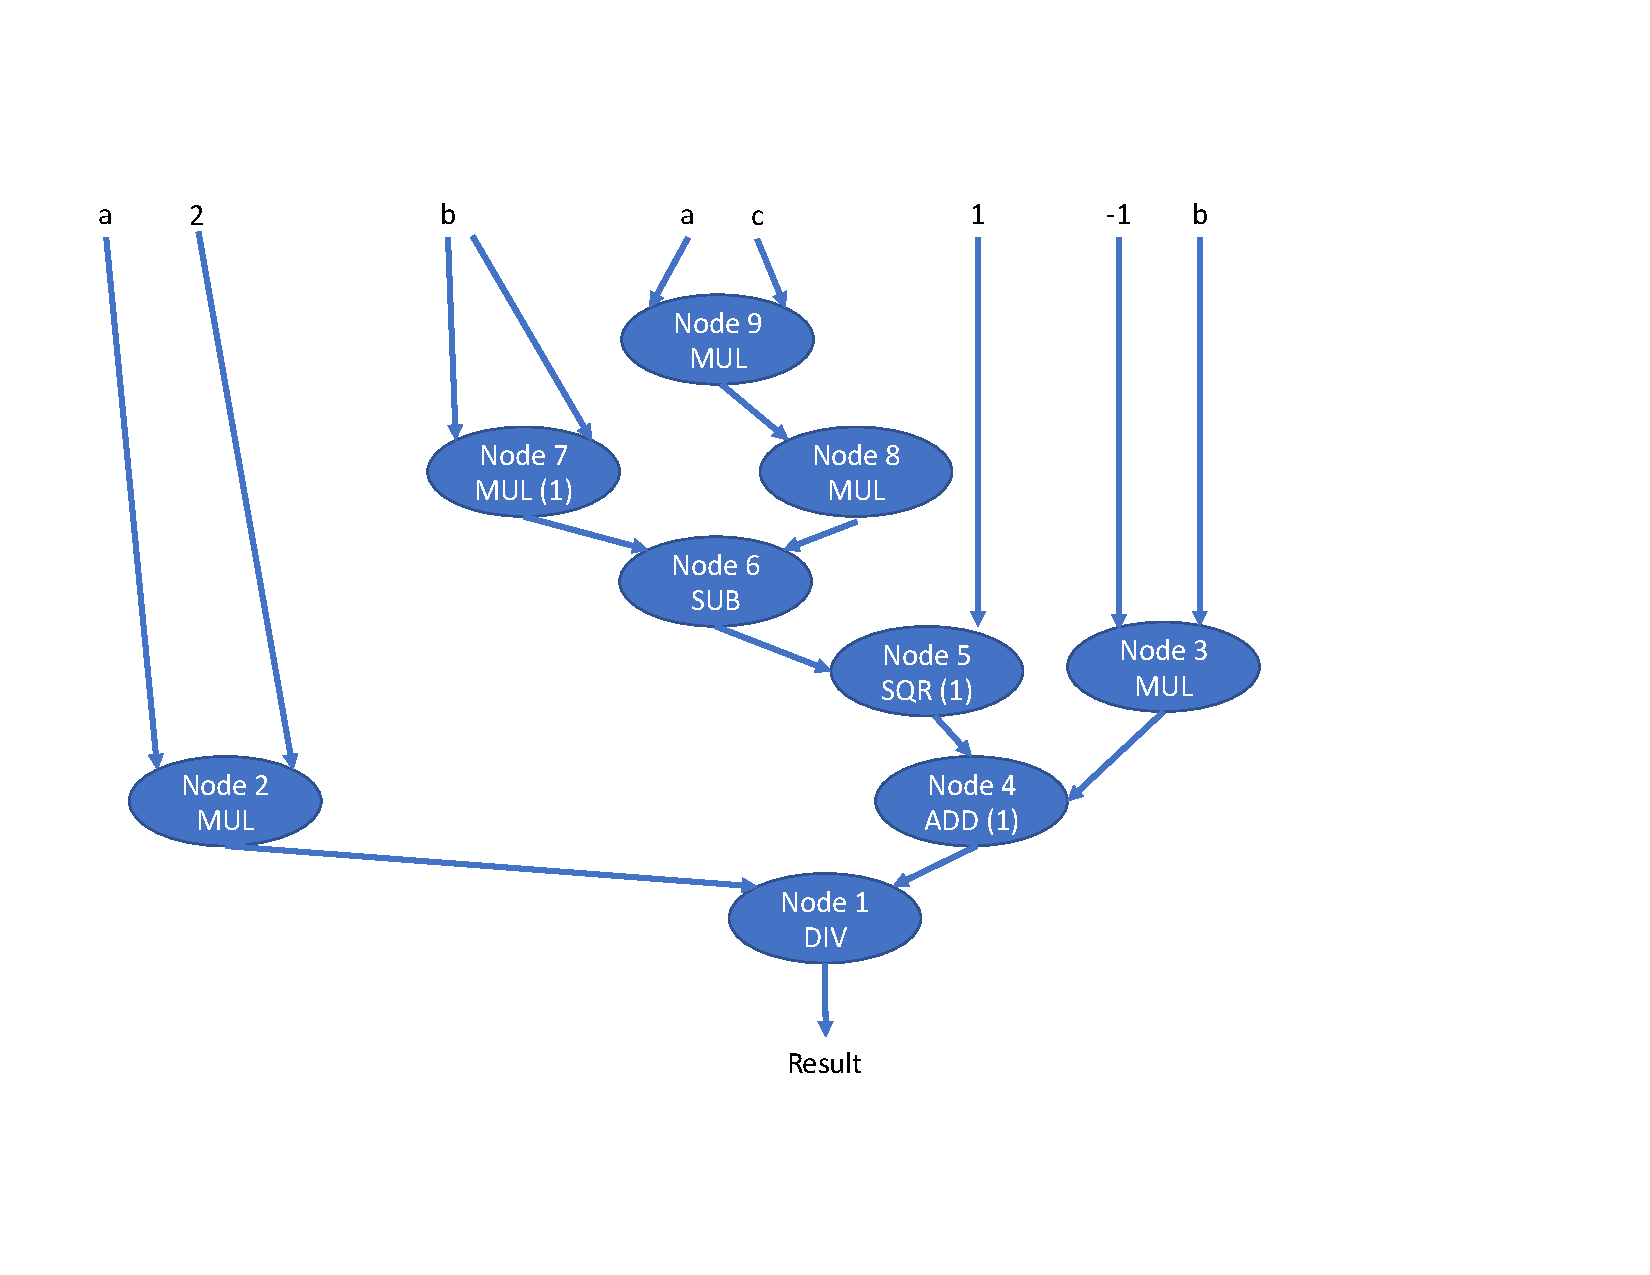
\includegraphics[scale=0.5]{quad.pdf}
\caption{Graphical representation of quadratic formula (the +SQR() root only).\label{fig:quad}}
\end{figure}

The key-value arguments to \verb+dfaddnode+ are
\begin{itemize}
\item \verb+-W woofname+ Gives the prefix for the \verb+.dfprogram+ and
\verb+.dfoperand+ WooFs.
\item \verb+-i node-id+ Each node in the DAG needs to be given a unique
integer identifier which is specified by the \verb+-i+ argument.
\item \verb+-o operation code+ Each operation that can be represented
by a node in the DAG is represented by an integer ``op code.''  When a node is
``fired'' the ``op code'' indexes a set of functions that perform
corresponding functions.    
\item \verb+-d dest-node-id+ After a node has ``fired'' (its operation
has been performed) the \verb+-d+ argument indicates the node-id that will
receive its output as an input.
\item \verb+-1 <optional>+ If the node that will receive the output of the
this node is not commutative, then make the output the first (left) input of
the destination node.
\end{itemize}
A \verb+dest-node-id+ of $0$ indicates the result of the computation.  

Recall, that \verb+dfoperand+ specifies edges that are inputs to the program
(i.e. edge that do not have a program node as a source). 
The key-value arguments for \verb+dfaddoperand+ are
\begin{itemize}
\item \verb+-W woofname+ Gives the prefix for the \verb+.dfprogram+ and 
\verb+.dfoperand+ WooFs.
\item \verb+-d dest-node-id+ The nodes that will receive the edge value
\item \verb+-1 <optional>+ If the node that will receive the output of the 
this node is not commutative, then make the output the first (left) input of 
the destination node.
\end{itemize}

For example, Figure~\ref{fig:quad} shows the DAG representation of the textual
representation shown in Listing~\ref{lst:quad}.
In the figure, inputs to the program (each defined by a \verb+dfaddoperand+
command) are shown along the top.  For clarity, each input is shown above
where it is consumed by a node and not with fan-out.  
That is, the ``a'' value and the ``b'' value are inputs to multiple nodes.
Also, the $(1)$ indicates non-commutative input.  For example, $Node 1$ (which
is a division operation) divides its first input (from $Node 4$ indicated by
$(1)$) by its second input (from $Node 2$).


\section{The CSPOT Dataflow Implementation}

The code that this section describes is contained in \verb+df.h+,
\verb+dfhandler.c+, and \verb+dfoperation.c+.  The latter contains the function
\verb+dfOperation()+
that maps node op codes to double precision arithmetic operations which it then performs
and returns.

Each element of the \verb+.dfprogram+ WooF has the following C-language
structure:
\begin{lstlisting}[language=C,caption={C structure for node WooF},label={lst:node}]
#define WAITING (0)
#define CLAIM (1)
#define DONE (2)

struct df_node_stc
{
        int opcode;     /* this op code */
        int ready_count;/* how many have we received */
        double value;   /* value of first operand to arrive */
        int order;      /* is waiting first or second in non-commute */
        int node_no;    /* which node is it */
        int dst_opcode; /* next node type */
        int dst_no;     /* next node address */
        int dst_order;  /* for non-commutative operations */
        int state;      /* waiting, claimed, done */
};
\end{lstlisting}
The constants \verb+WAITING+, \verb+CLAIM+, and \verb+DONE+ are the values
that the \verb+state+ field.  The program \verb+dfaddnode+ initializes and
then appends to the program WooF one of these structures for each node in a
program.  The initial value of \verb+ready_count+ is $0$ and the initial state
is \verb+WAITING+.  The put operation in \verb+dfaddnode+ that appends each
structure does not trigger a handler.

The operand structure is shown in the following listing:
\begin{lstlisting}[language=C,caption={C structure for operand WooF},label={lst:operand}]
struct df_operand_stc
{
        double value;           /* operand value */
        int dst_no;             /* dest node address */
        int order;              /* for non-commute */
        char prog_woof[1024];   /* name of woof holding the program */
};
\end{lstlisting}
The program \verb+dfaddoperand+ appends one of these structures for each
program input to the \verb+.dfoperand+ WooF.  Each put operation in
\verb+dfaddoperand+ specifies the handler \verb+dfhandler+ which implements
dataflow execution cycle. 

The \verb+dfhandler+ CSPOT handler is invoked on the \verb+dfoperand+ WooF
every time an operand is appended to the \verb+.dfoperand+ WooF.  On handler
entry, it initializes a node structure for the destination node and the state
set to \verb+CLAIM+ that it then appends to the program WooF.  The purpose of
this node is to set the sequence number (held in the \verb+c_seqno+ 
variable) that defines the place in the log that begins a backward scan
of the program WooF.

The handler then scans backwards (from \verb+c_seqno-1+) through the program
WooF looking for a node that has a \verb+node_id+ equal to the \verb+node_id+
in the \verb+CLAIM+ node (which is the same as the \verb+dest_node_id+ in the
operand).  If it finds a matching node, then the \verb+ready_count+ value is
either $0$ (and the state is \verb+WAITING+) indicating that the node has yet
to receive either input or the \verb+ready_count+ is $1$ (state also
\verb+WAITING+) indicating that the
node is ``partially fired'' by having one of its two inputs delivered.

If \verb+ready_count+ is $1$ (and the \verb+node_id+ matches), then 
the node has already received its first operand and the handler must fire the
node.  To do so, it takes the value (passed in the operand structure to the
handler) and the value stored in the node when it was partially fired passes
the two of them to the function \verb+dfOperation()+ 
(possibly ordering the inputs
if the flag indicating a non-commutative operation is set) 
which applies the op code in
the node to the two inputs and returns the double precision result.  It then
calls the \verb+dfFireNode()+ function to fire the node and pass its result to its
destination node.

The \verb+dfFireNode()+ function sets the node's state to \verb+DONE+ and its
\verb+ready_count+ to $2$ (since both inputs are present).  It puts this
``DONE'' node into the node WooF largely for debugging purposes since a node
marked \verb+DONE+ has a \verb+ready_count+ of $2$ and hence will be skipped
by the handler in any node WooF scan.

The \verb+dfFireNode()+ function also initializes an operand structure for the
result computed by the node, sets the \verb+dst_no+ id to be the node id of
the destination node that is to receive this result as an input, and appends
the new operand to the operand WooF, specifying \verb+dfhandler+ in the put
(triggering a handler invocation for this operand).

Each append to the operand WooF, then, triggers another handler that moves the
destination node through the execution cycle.

The \verb+dfFireNode()+ function is only called when the second node input
arrives.  When the first input arrives, the handler looks for a matching node
that has a state set to \verb+CLAIM+ and a sequence number (in the program
WooF) smaller than \verb+c_seqno+.  If it finds such a record, then an
``older'' claim is underway (another handler is running for the node with
\verb+node_id+).  The logic is that this older handler invocation should
continue and then rescan from the new end of the program WooF looking for the
younger \verb+CLAIM+ node.  That is, if two handlers run for the same node,
their respective \verb+CLAIM+ records will append to the WooF with one
occurring before the other.  The first one (the one with a smaller sequence
number) will take the \verb+ready_count+ from $0$ to $1$ creating a partially
fired node \textit{and then} scan backwards looking for the younger
\verb+CLAIM+ record.  If it finds a second \verb+CLAIM+ then the older handler
completes the node's firing.  Thus, the handler appending the younger
\verb+CLAIM+ simply exits, leaving the older hander to handle both the partial
fire and the complete fire of the node.

Thus, when a partial fire occurs (when the original node WooF scan finds a
\verb+ready_count+ set to $0$) it puts a node to the program WooF with the
\verb+ready_count+ set to $1$ (indicating a partial fire).  It then scans
the node WooF backwards from the sequence number for the partial fire to the
sequence number for the older \verb+CLAIM+ node (contained in \verb+c_seqno+).
If it finds a another \verb+CLAIM+ in the sequence number range between the
partial fire and the original \verb+CLAIM+ then a second handler executed later
and exited.  This handler, then fires the node by calling \verb+dfOperation()+
to compute the result, and \verb+df_fire_node()+ as described above.  If a second
\verb+CLAIM+ node is not found during this scan, then the handler exits and a
subsequent handler invocation will find the partial fire in the node WooF and
complete the node's firing.

\section{Some Thoughts}

The prototype demonstrates that it is possible to implement dataflow
relatively efficiently using the current definition of CSPOT.  The log scan
for a node with \verb+ready_count = 0+ is $O(n)$ where there are $n$ program
nodes, however if the nodes are added to the program WooF from top to bottom,
the actual scan is much less.  Scans for partially fired nodes are $O(k)$
where $k$ is the make span of the program graph (assuming the DONE nodes are
removed).  Finally, handlers that are
not associated with dependent nodes can execute in parallel.
However the prototype is otherwise not terribly useful.  There are
several extensions that are possible that are likely fruitful areas of study.

One extension is to change the arity of the nodes from $2$ to some arbitrary
maximum.  The handler would need to become more complex since a partially
fired node would be any node with at least $1$ input available that is not
DONE.  However, this change would allow a compiler or runtime system to
``coalesce'' fine-grained nodes into coarser nodes.  That is, the prototype
does a great deal of work to execute a single double-precision arithmetic
operation.  A ``true'' system would bundle multiple such operations together
to save the overhead.

A second, related, extension is to allow for arbitrary functional operations
(as opposed to double-precision arithmetic).  Here the issue is that the
operand WooF will need to have elements that are sized by the C union of
\textit{all} possible node inputs.  There are several ways to implement this
extension, but all of them make the simple API (consisting of \verb+dfinit+,
\verb+dfaddnode+, and \verb+dfaddoperand+) considerably more complex.  Still,
this complexity is properly part of the intermediate representation and could
be managed by a full-fledged language system.

Another set of extensions is to add iteration and conditionals to the dataflow
language.  A simple way to do so is to embed this functionality in bash or
what ever scripting language is calling the dataflow API.  The challenge with
this approach is primarily loop-carried dependencies.  That is, the output of
a node in one iteration may be an input to a node in another and there is not
a way in the API to express this kind of dependency.  

One way to achieve this functionality is to change the current prototype so
that the program nodes for each loop body each go in a new program WooF.
Similarly, the start of each loop body would also require a new operand WooF
that carries program inputs and also dependencies from previous loop bodies.   

Architecturally, the change would likely split the program WooF into a ``code''
WooF (that contains the program nodes) and a ``state'' WooF that contains
partially fired nodes, CLAIM records, etc.  There would be one code WooF for
the loop body, but each iteration gets its own (or a reinitialized) state
WooF.  Each loop body will also require its own operand WooF which would need
to be created as soon as a loop body result is generated.  

Lastly, the current system is not distributed.  That is, the \verb+dfinit+
function creates an operand WooF and a program WooF in the same CSPOT
namespace.  The operand WooF does have the program WooF's URI in it so that
nodes could be fired ion other namespaces, but the dataflow API does not have
an option for adding a namespace URI to each node.  If the API allowed a URI
for every destination node, then it would be possible to execute functions
remotely from the location of the operand WooF.

Distributing the operand WooFs is slightly more complex.  The initial operands
would specify target namespaces but the API would need a URI for the output of
each node specifying an operand WooF which would then carry a separate URI for
the target node.

In short, the model is distributed, but implementing it using the current
prototype makes the prototype dataflow API quite unruly due to the need to
specify URIs for nodes and operands.  Most likely, the approach in the
prototype would ultimately result in an IR that a language system or visual
programming system would emit.  If that is true, than a redesign of the
dataflow API (to make it more of an IR) is probably the right thing to do.



\end{document}

